\chapter{Regular Surfaces}\label{chap:surfaces}

% ==================== Section 2-1: Introduction ====================
\section{Introduction}\label{sec:surfaces-intro}

\textbf{From curves to surfaces.} 在第一章中，我们研究了 $\mathbb{R}^3$ 中的曲线理论。通过引入曲率和挠率，我们学会了如何用精确的数学语言描述曲线的"弯曲程度"。自然的问题是：能否将类似的理论推广到二维甚至更高维的对象？

这一想法引导我们进入曲面理论。与曲线不同的是，曲面是"二维"的——它们在每一点附近都像一个平面。正如曲线需要正则性（避免尖点）以便定义切线，曲面也需要某种正则性条件以保证切平面（tangent plane）的存在。

\textbf{The main theme.} 本章研究 $\mathbb{R}^3$ 中曲面的微分几何。我们将看到，曲面为二元函数的微积分提供了天然的研究框架。事实上，曲面论正是高斯（Gauss）和黎曼（Riemann）开创现代微分几何的起点。

\textbf{Organization of this chapter.} 本章内容安排如下。2-2 节引入正则曲面（regular surface）的基本概念，这是全书的基础；2-3 节讨论曲面上的可微函数；2-4 节引入第一基本形式（first fundamental form），用于处理曲面上的度量问题（弧长、面积等）。

\textbf{Why surfaces?} 曲面之所以重要，有多重原因。首先，现实世界中的许多物体（地球表面、电影屏幕、弯曲的镜片）都是曲面而非曲线。其次，曲面理论是理解弯曲空间（曲面的内蕴几何）的起点——高斯称之为"非凡的定理"（Theorema Egregium）：曲面的曲率可以仅用曲面自身的度量来定义，而不依赖于它如何嵌入 $\mathbb{R}^3$。这一发现深刻地影响了物理学中广义相对论的发展。

\begin{figure}[H]
\centering
\begin{minipage}{0.45\textwidth}
\centering
\subfloat[Figure 2-1. 正则曲面的参数化]{\label{fig:fig2-1}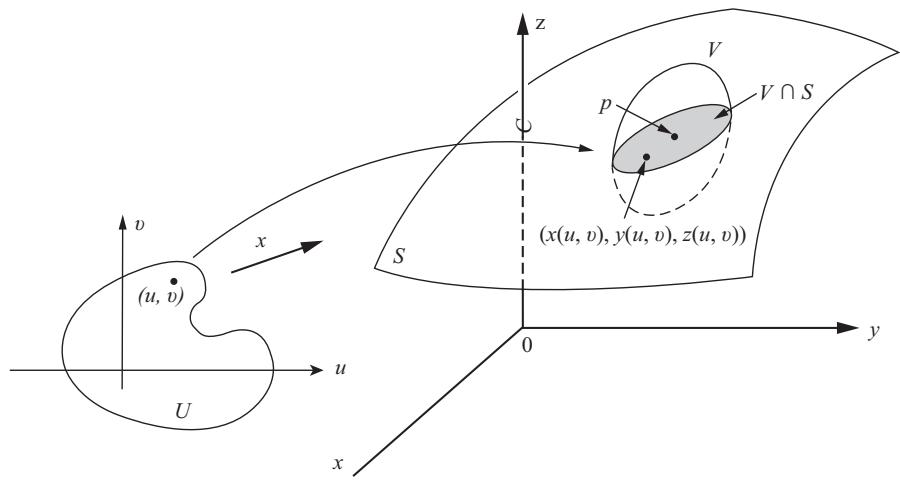
\includegraphics[width=\textwidth]{../../../../PDFs/differential-geometry/transcript/Do Carmo - Differential Geometry of Curves and Surfaces/hybrid_ocr/images/9182b715913ef41534ac27f5769d97aea20063b58fd9d15ca1b4ef11da858ff1.jpg}}
\end{minipage}
\hfill
\begin{minipage}{0.45\textwidth}
\centering
\subfloat[Figure 2-2. 坐标曲线与切向量]{\label{fig:fig2-2}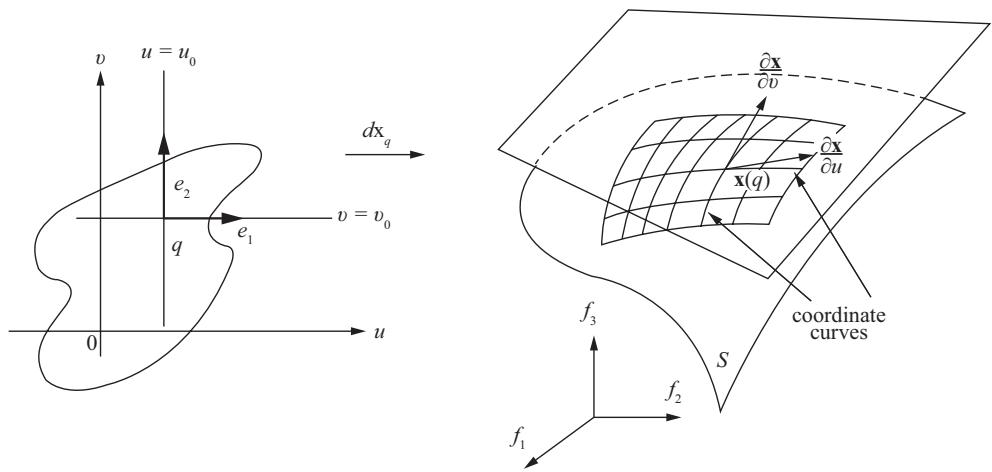
\includegraphics[width=\textwidth]{../../../../PDFs/differential-geometry/transcript/Do Carmo - Differential Geometry of Curves and Surfaces/hybrid_ocr/images/14fe34e73ea93e0d8038fe79aff12b40bf5ece89780624d7e112f6143d6d1a63.jpg}}
\end{minipage}
\end{figure}

% ==================== Section 2-2: Regular Surfaces ====================
\section{Regular Surfaces; Inverse Images of Regular Values}\label{sec:regular-surfaces}

\textbf{Defining a surface.} 如何精确地定义"曲面"？直观上，曲面是 $\mathbb{R}^3$ 中的一块"二维"片状结构，它没有尖点、没有自交，并且在每一点处都有良好的切平面。

与曲线的定义方式不同（曲线是参数化映射），我们定义曲面为 $\mathbb{R}^3$ 的一个子集。原因是：曲面作为"面"，应该是独立于参数化而存在的几何对象。

\begin{Definition}[正则曲面]\label{def:regular-surface}
设 $S \subset \mathbb{R}^3$。如果对每一点 $p \in S$，存在 $\mathbb{R}^3$ 中的邻域 $V$ 和映射
\[
\mathbf{x}: U \subset \mathbb{R}^2 \to V \cap S,
\]
其中 $U$ 是 $\mathbb{R}^2$ 中的开集，使得（见 \cref{fig:fig2-1}，教材 Figure 2-1）：
\begin{enumerate}
\item $\mathbf{x}$ 是可微的。这意味着如果写
\[
\mathbf{x}(u,v) = (x(u,v), y(u,v), z(u,v)),\quad (u,v) \in U,
\]
则函数 $x(u,v), y(u,v), z(u,v)$ 在 $U$ 上有所有阶的连续偏导数。

\item $\mathbf{x}$ 是同胚。即 $\mathbf{x}$ 连续且有连续的逆映射 $\mathbf{x}^{-1}: V \cap S \to U$。

\item（正则条件）对每个 $q \in U$，微分 $d\mathbf{x}_q: \mathbb{R}^2 \to \mathbb{R}^3$ 是单射。
\end{enumerate}
则称 $S$ 为\textbf{\underline{正则曲面}}（regular surface）。
\end{Definition}

映射 $\mathbf{x}$ 称为 $p$ 邻域的\textbf{\underline{参数化}}（parametrization）或\textbf{\underline{局部坐标}}（system of (local) coordinates）。

\textbf{The regularity condition.} 条件 3 至关重要。回顾：$d\mathbf{x}_q$ 在标准基下的矩阵为
\[
d\mathbf{x}_q = \begin{pmatrix}
\frac{\partial x}{\partial u} & \frac{\partial x}{\partial v} \\
\frac{\partial y}{\partial u} & \frac{\partial y}{\partial v} \\
\frac{\partial z}{\partial u} & \frac{\partial z}{\partial v}
\end{pmatrix}.
\]

条件 3 要求这两列向量线性无关——即向量 $\partial\mathbf{x}/\partial u$ 和 $\partial\mathbf{x}/\partial v$ 不平行。几何上，这意味着在 $p$ 点处存在良好定义的切平面。

\begin{Remark}
让我们逐一解释这三个条件的几何意义：
\begin{itemize}
\item 条件 1（可微性）保证曲面是"光滑"的，能够进行微分运算；
\item 条件 2（单射性）防止自交——如果曲面与自身相交，就无法谈论"在 $p$ 点的切平面"；
\item 条件 3（正则条件）保证每点都有良好定义的切平面。
\end{itemize}
这三个条件共同确保了曲面上的微分几何是有意义的。
\end{Remark}

\begin{figure}[H]
\centering
\begin{minipage}{0.45\textwidth}
\centering
\subfloat[Figure 2-3 (a). 自交情形 — 不能定义唯一切平面]{\label{fig:fig2-3a}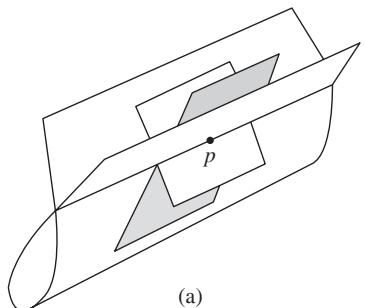
\includegraphics[width=\textwidth]{../../../../PDFs/differential-geometry/transcript/Do Carmo - Differential Geometry of Curves and Surfaces/hybrid_ocr/images/982f74acb26628a48d71a466dae574fef45a04dbcf320fcb5714a526f10cd8ed.jpg}}
\end{minipage}
\hfill
\begin{minipage}{0.45\textwidth}
\centering
\subfloat[Figure 2-3 (b). 正则曲面 — 每点有良好定义的切平面]{\label{fig:fig2-3b}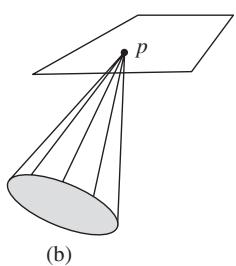
\includegraphics[width=\textwidth]{../../../../PDFs/differential-geometry/transcript/Do Carmo - Differential Geometry of Curves and Surfaces/hybrid_ocr/images/0020313622314d0c333e47f99980b4ef05e0c8ac53e5c0910d29805904e23797.jpg}}
\end{minipage}
\end{figure}

\begin{Example}[单位球面]\label{ex:sphere}
单位球面
\[
S^2 = \{(x,y,z) \in \mathbb{R}^3; x^2 + y^2 + z^2 = 1\}
\]
是正则曲面。

我们用六个参数化来覆盖整个球面。例如，定义 $\mathbf{x}_1: U \subset \mathbb{R}^2 \to \mathbb{R}^3$ 为
\[
\mathbf{x}_1(x,y) = (x, y, +\sqrt{1-(x^2+y^2)}),\quad (x,y) \in U,
\]
其中 $U = \{(x,y) \in \mathbb{R}^2; x^2 + y^2 < 1\}$。

验证三个条件：
\begin{enumerate}
\item $\mathbf{x}_1$ 是可微的（因为 $x^2+y^2<1$ 时根号内为正）；
\item $\mathbf{x}_1$ 是单射，逆映射是投影 $\pi(x,y,z) = (x,y)$；
\item 雅可比行列式 $\frac{\partial(x,y)}{\partial(x,y)} \equiv 1 \neq 0$。
\end{enumerate}

类似地定义 $\mathbf{x}_2$（下半球）、$\mathbf{x}_3, \mathbf{x}_4$（$xz$ 平面投影）、$\mathbf{x}_5, \mathbf{x}_6$（$yz$ 平面投影），这六个参数化共同覆盖整个球面（见 \cref{fig:fig2-4}，教材 Figure 2-4）。
\end{Example}

\begin{figure}[H]
\centering
\begin{minipage}{0.7\textwidth}
\centering
\subfloat[Figure 2-4. 球面的六个参数化邻域]{\label{fig:fig2-4}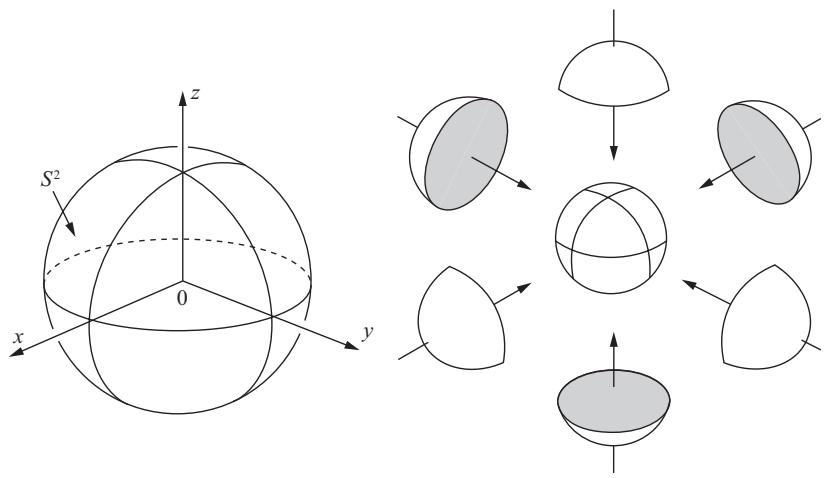
\includegraphics[width=\textwidth]{../../../../PDFs/differential-geometry/transcript/Do Carmo - Differential Geometry of Curves and Surfaces/hybrid_ocr/images/b0f439063c9a3837b427e9f827366c854cdb5ae59b8c0eb305664cba91fa43a6.jpg}}
\end{minipage}
\end{figure}

\textbf{Geographical coordinates.} 对于大多数应用，更方便的是使用球面坐标。设
\[
V = \{(\theta, \varphi); 0 < \theta < \pi,\; 0 < \varphi < 2\pi\},
\]
定义 $\mathbf{x}: V \to \mathbb{R}^3$ 为（见 \cref{fig:fig2-5}，教材 Figure 2-5）
\[
\mathbf{x}(\theta, \varphi) = (\sin\theta\cos\varphi,\; \sin\theta\sin\varphi,\; \cos\theta).
\]
这里 $\theta$ 是余纬度（colatitude），$\varphi$ 是经度（longitude）。
\begin{figure}[H]
\centering
\begin{minipage}{0.5\textwidth}
\centering
\subfloat[Figure 2-5. 球面坐标 $\theta$ 和 $\varphi$]{\label{fig:fig2-5}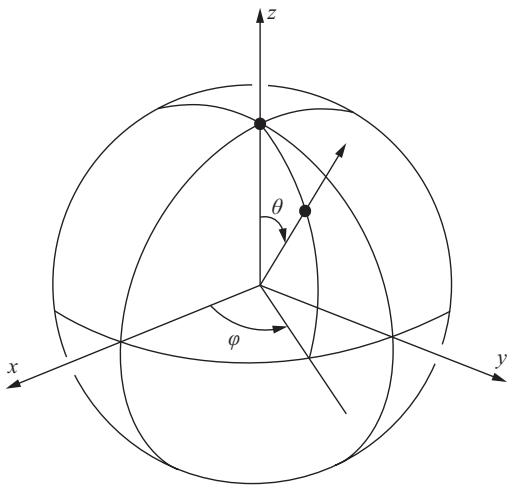
\includegraphics[width=\textwidth]{../../../../PDFs/differential-geometry/transcript/Do Carmo - Differential Geometry of Curves and Surfaces/hybrid_ocr/images/29b4cf1487ab401a9c3132cb791f96ac850e3b26e7a0a1b77ea146f3315d284b.jpg}}
\end{minipage}
\end{figure}

\begin{Proposition}[垂直投影判断法]\label{prop:graph-criterion}
设 $S \subset \mathbb{R}^3$。如果对每一点 $p \in S$，存在 $p$ 的邻域 $V$ 使得 $V \cap S$ 是以下三种形式之一：
\[
z = f(x,y),\quad y = g(x,z),\quad x = h(y,z),
\]
其中 $f,g,h$ 是可微函数，则 $S$ 是正则曲面。
\end{Proposition}

\textbf{Why is this useful?} 这个命题告诉我们：判断一个集合是否是曲面，只需检查它局部是否是某个可微函数的图像。这比直接验证定义中的三个条件要容易得多。

\begin{Example}[旋转面]\label{ex:surface-of-revolution}
设 $C$ 是 $xz$ 平面中的一条光滑曲线，绕 $z$ 轴旋转得到的曲面是正则曲面（如果 $C$ 不与 $z$ 轴相交）。例如，环面（torus）就是由椭圆绕 $z$ 轴旋转而成的。

旋转面的参数化可以写成
\[
\mathbf{x}(u,v) = ((r\cos u + a)\cos v,\; (r\cos u + a)\sin v,\; r\sin u),
\]
其中 $0 < u, v < 2\pi$（见 \cref{fig:fig2-9}，教材 Figure 2-9）。
\end{Example}

\begin{figure}[H]
\centering
\begin{minipage}{0.6\textwidth}
\centering
\subfloat[Figure 2-9. 环面 (torus)]{\label{fig:fig2-9}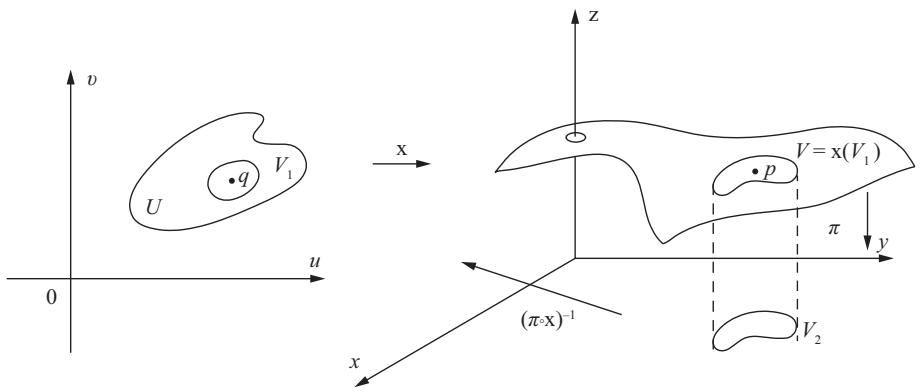
\includegraphics[width=\textwidth]{../../../../PDFs/differential-geometry/transcript/Do Carmo - Differential Geometry of Curves and Surfaces/hybrid_ocr/images/abf059759e9ec36e5b4e3fdbafd96373e1127c14a7e600e0f029e4745e090361.jpg}}
\end{minipage}
\end{figure}

\begin{Example}[锥面不是正则曲面]\label{ex:cone-not-regular}
单叶锥面
\[
C = \{(x,y,z) \in \mathbb{R}^3; z = +\sqrt{x^2+y^2}\}
\]
\textbf{不是}正则曲面。关键在于顶点 $(0,0,0)$ 处——任何包含该点的邻域都与锥面相交，而在该点处无法定义良好的切平面（锥面在顶点处有一个"尖"）。

这个例子说明了定义中条件 3 的必要性：如果仅仅去掉顶点，修改后的曲面将是正则的。
\end{Example}

\subsection*{2-2 节练习}

\begin{exercise}{2-2, 1 — do Carmo, Exercise 2-2, 1}
Show that the cylinder $\{(x,y,z)\in \mathbb{R}^3;x^2 +y^2 = 1\}$ is a regular surface, and find parametrizations whose coordinate neighborhoods cover it.
\end{exercise}

\begin{exercise}{2-2, 2 — do Carmo, Exercise 2-2, 2}
Is the set $\{(x,y,z)\in \mathbb{R}^3;z = 0$ and $x^{2} + y^{2}\leq 1\}$ a regular surface? Is the set $\{(x,y,z)\in \mathbb{R}^3;z = 0$, and $x^{2} + y^{2} < 1\}$ a regular surface?
\end{exercise}

\begin{exercise}{2-2, 3 — do Carmo, Exercise 2-2, 3}
Show that the two-sheeted cone, with its vertex at the origin, that is, the set $\{(x,y,z)\in \mathbb{R}^3;x^2 +y^2 -z^2 = 0\}$, is not a regular surface.
\end{exercise}

\begin{exercise}{2-2, 4 — do Carmo, Exercise 2-2, 4}
Let $f(x, y, z) = z^2$. Prove that $0$ is not a regular value of $f$ and yet that $f^{-1}(0)$ is a regular surface.
\end{exercise}

\begin{exercise}{2-2, 5* — do Carmo, Exercise 2-2, 5}
Let $P = \{(x, y, z) \in \mathbb{R}^3; x = y\}$ (a plane) and let $\mathbf{x}: U \subset \mathbb{R}^2 \to \mathbb{R}^3$ be given by
\[
\mathbf{x}(u, v) = (u + v, u + v, uv),
\]
where $U = \{(u,v)\in \mathbb{R}^2;u > v\}$. Clearly, $\mathbf{x}(U)\subset P$. Is $\mathbf{x}$ a parametrization of $P$?
\end{exercise}

\begin{exercise}{2-2, 6 — do Carmo, Exercise 2-2, 6}
Give another proof of Prop. 1 by applying Prop. 2 to $h(x, y, z) = f(x, y) - z$.
\end{exercise}

\begin{exercise}{2-2, 7 — do Carmo, Exercise 2-2, 7}
Let $f(x, y, z) = (x + y + z - 1)^2$.
\begin{enumerate}
\item[a.] Locate the critical points and critical values of $f$.
\item[b.] For what values of $c$ is the set $f(x, y, z) = c$ a regular surface?
\item[c.] Answer the questions of parts a and b for the function $f(x, y, z) = xyz^2$.
\end{enumerate}
\end{exercise}

\begin{exercise}{2-2, 8* — do Carmo, Exercise 2-2, 8}
Let $\mathbf{x}(u, v)$ be as in Def. 1. Verify that $d\mathbf{x}_q: \mathbb{R}^2 \to \mathbb{R}^3$ is one-to-one if and only if
\[
\frac{\partial \mathbf{x}}{\partial u} \wedge \frac{\partial \mathbf{x}}{\partial v} \neq 0.
\]
\end{exercise}

\begin{exercise}{2-2, 9 — do Carmo, Exercise 2-2, 9}
Let $V$ be an open set in the $xy$ plane. Show that the set
\[
\{(x, y, z) \in \mathbb{R}^3; z = 0 \text{ and } (x, y) \in V\}
\]
is a regular surface.
\end{exercise}

\begin{exercise}{2-2, 10* — do Carmo, Exercise 2-2, 10}
Let $C$ be a figure "8" in the $xy$ plane and let $S$ be the cylindrical surface over $C$ (见 \cref{fig:fig2-11}，教材 Figure 2-11); that is,
\[
S = \{(x, y, z) \in \mathbb{R}^3; (x, y) \in C \}.
\]
Is the set $S$ a regular surface?
\end{exercise}

\begin{figure}[H]
\centering
\begin{minipage}{0.5\textwidth}
\centering
\subfloat[Figure 2-11. 8字曲线生成的柱面]{\label{fig:fig2-11}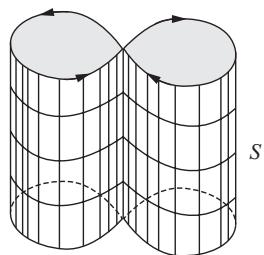
\includegraphics[width=\textwidth]{../../../../PDFs/differential-geometry/transcript/Do Carmo - Differential Geometry of Curves and Surfaces/hybrid_ocr/images/989523d17639b5f31f0ed0e2d4d9077a348942766a19d1143dd29cf290eae71d.jpg}}
\end{minipage}
\end{figure}

% ==================== Section 2-3: Change of Parameters ====================
\section{Change of Parameters; Differentiable Functions on Surfaces}\label{sec:change-of-params}

在上一节中，我们看到正则曲面可以用不同的参数化来描述。例如，球面可以用地理坐标 $(\theta, \varphi)$，也可以用平面垂直投影的六个局部坐标卡来描述。重要的是，**由曲面本身决定的几何量**（如切平面）不应该依赖于参数化的选择。

\textbf{Why do we need different parametrizations?} 一个参数化 $\mathbf{x}: U \to S$ 只能覆盖曲面的一部分。例如，球面的地理坐标参数化在两极处失效（雅可比为零）。因此，我们需要多个参数化来覆盖整个曲面。

不同参数化之间的关系由**坐标变换**（change of parameters）描述。如果 $\mathbf{x}: U \to S$ 和 $\tilde{\mathbf{x}}: \tilde{U} \to S$ 是两个有重叠区域的参数化，则在重叠区域上有坐标变换
\[
\Phi = \mathbf{x}^{-1} \circ \tilde{\mathbf{x}}: \tilde{U}' \to U,
\]
其中 $\tilde{U}' \subset \tilde{U}$ 是重叠区域在 $\tilde{\mathbf{x}}$ 下的像。

\begin{Proposition}[坐标变换是可微的]\label{prop:change-of-params}
设 $\mathbf{x}: U \to S$ 和 $\tilde{\mathbf{x}}: \tilde{U} \to S$ 是正则曲面 $S$ 的两个参数化，假设 $\mathbf{x}^{-1}(\mathbf{x}(U) \cap \tilde{\mathbf{x}}(\tilde{U})) \subset U$。则坐标变换 $\Phi = \mathbf{x}^{-1} \circ \tilde{\mathbf{x}}$ 是可微的。
\end{Proposition}

\textbf{This is important.} 这个命题告诉我们：无论我们用哪个参数化来计算，曲面上的可微函数的概念是良好定义的。一个函数 $f: S \to \mathbb{R}$ 在点 $p$ 处可微，意味着它在某个（从而任何）参数化下是可微的。

\begin{Definition}[曲面上的可微函数]\label{def:differentiable-function-on-surface}
设 $f: S \to \mathbb{R}$ 是定义在正则曲面 $S$ 上的函数。如果对每一点 $p \in S$，存在参数化 $\mathbf{x}: U \to S$ 使得 $p \in \mathbf{x}(U)$，且合成函数
\[
f \circ \mathbf{x}: U \subset \mathbb{R}^2 \to \mathbb{R}
\]
在 $q = \mathbf{x}^{-1}(p)$ 处是可微的，则称 $f$ 在 $p$ 处\textbf{\underline{可微}}（differentiable）。
\end{Definition}

类似地，可以定义可微映射 $F: S_1 \to S_2$。

\begin{Remark}
这个定义的关键在于：它不依赖于参数化的选择。如果一个函数在一个参数化下是可微的，它在所有参数化下都是可微的。
\end{Remark}

\begin{Example}[高度函数]\label{ex:height-function}
设 $S$ 是单位球面，定义高度函数 $f: S \to \mathbb{R}$ 为 $f(x,y,z) = z$。在地理坐标下，$f(\mathbf{x}(\theta,\varphi)) = \cos\theta$，这是可微的。因此 $f$ 是 $S$ 上的可微函数。
\end{Example}

\begin{Definition}[可微曲线]\label{def:differentiable-curve-on-surface}
曲面 $S$ 上的\textbf{可微曲线}是可微映射 $\alpha: I \subset \mathbb{R} \to S$，其中 $I$ 是区间。
\end{Definition}

\textbf{Connection with Chapter 1.} 注意到如果 $\alpha: I \to S$ 是曲面 $S$ 上的可微曲线，则作为 $\mathbb{R}^3$ 中的曲线，$\alpha$ 也是可微的（因为包含映射 $i: S \hookrightarrow \mathbb{R}^3$ 是嵌入）。

\subsection*{2-3 节练习}

\begin{exercise}{2-3, 1 — do Carmo, Exercise 2-3, 1}
Let $S^2 = \{(x,y,z) \in \mathbb{R}^3; x^2 + y^2 + z^2 = 1\}$ be the unit sphere and let $f: S^2 \to \mathbb{R}$ be given by $f(x,y,z) = z$. Show that $f$ is differentiable.
\end{exercise}

\begin{exercise}{2-3, 2 — do Carmo, Exercise 2-3, 2}
Let $S \subset \mathbb{R}^3$ be a regular surface and let $p \in S$. Show that there exists a neighborhood $V$ of $p$ in $S$ such that the projection onto the tangent plane at $p$ maps $V$ diffeomorphically onto an open set of $\mathbb{R}^2$.
\end{exercise}

\begin{exercise}{2-3, 3* — do Carmo, Exercise 2-3, 3}
Let $\mathbf{x}: U \to S$ be a parametrization of a regular surface $S$. Show that $\mathbf{x}^{-1}: \mathbf{x}(U) \to U$ is continuous. (This shows that condition 2 in the definition of a regular surface can be replaced by: $\mathbf{x}$ is a homeomorphism onto its image.)
\end{exercise}

\begin{exercise}{2-3, 4 — do Carmo, Exercise 2-3, 4}
Let $F: S_1 \to S_2$ be a differentiable map between regular surfaces. Show that the set of critical points of $F$ is closed in $S_1$.
\end{exercise}

\begin{exercise}{2-3, 5 — do Carmo, Exercise 2-3, 5}
Show that the map $F: S^2 \to S^2$ given by $F(x,y,z) = (-x,y,z)$ (a rotation by $\pi$ around the $y$-axis) is differentiable. Find the matrix of $dF_p$ in an appropriate basis.
\end{exercise}

% ==================== Section 2-4: The Differential of a Map ====================
\section{The Differential of a Map; Tangent Plane}\label{sec:differential-tangent-plane}

\textbf{From curves to surfaces.} 在第一章中，我们看到曲线的切向量是导数 $\alpha'(t)$。对于曲面之间的可微映射，我们可以类似地定义微分（differential），它描述了映射在一点处的线性近似。

关键问题是：如何定义曲面的切平面？如果曲面 $S$ 是参数化曲面 $\mathbf{x}: U \to \mathbb{R}^3$ 的像，那么切平面应该由 $\partial\mathbf{x}/\partial u$ 和 $\partial\mathbf{x}/\partial v$ 张成。

\begin{Definition}[切向量]\label{def:tangent-vector-surface}
设 $p \in S$。向量 $v \in \mathbb{R}^3$ 称为 $S$ 在 $p$ 处的\textbf{\underline{切向量}}（tangent vector），如果存在可微曲线 $\alpha: (-\epsilon, \epsilon) \to S$ 使得 $\alpha(0) = p$，$\alpha'(0) = v$。
\end{Definition}

$S$ 在 $p$ 处的所有切向量构成一个二维线性空间，称为\textbf{\underline{切空间}}（tangent space），记为 $T_pS$。

\begin{Proposition}[切空间的构造]\label{prop:tangent-space}
设 $\mathbf{x}: U \to S$ 是 $p = \mathbf{x}(q)$ 处的参数化。则
\[
T_pS = d\mathbf{x}_q(\mathbb{R}^2) = \text{span}\left\{\frac{\partial\mathbf{x}}{\partial u}(q),\; \frac{\partial\mathbf{x}}{\partial v}(q)\right\}.
\]
\end{Proposition}

这个命题告诉我们：切空间恰好是由参数化的两个偏导向量张成的平面。这正是我们直观上对切平面的期望。

\begin{Definition}[切平面]\label{def:tangent-plane}
正则曲面 $S$ 在点 $p$ 处的\textbf{\underline{切平面}}（tangent plane）是在 $p$ 处与 $S$ 相切且平行于 $T_pS$ 的平面。
\end{Definition}

\textbf{Geometric meaning.} 切平面的方程可以通过点 $p$ 和法向量 $N$ 来描述。我们稍后会看到如何计算 $N$。

\begin{Example}[球面的切平面]\label{ex:sphere-tangent-plane}
单位球面 $S^2$ 在点 $p = (x_0, y_0, z_0)$ 处的切平面由法向量 $p$（因为球面在每一点的法向量就是指向球心的向量）给出。切平面方程为
\[
x_0(x - x_0) + y_0(y - y_0) + z_0(z - z_0) = 0.
\]
\end{Example}

\begin{Definition}[可微映射的微分]\label{def:differential-map}
设 $F: S_1 \to S_2$ 是可微映射，$p \in S_1$。定义\textbf{微分} $dF_p: T_pS_1 \to T_{F(p)}S_2$ 如下：给定 $v \in T_pS_1$，取可微曲线 $\alpha: (-\epsilon, \epsilon) \to S_1$ 使得 $\alpha(0) = p$，$\alpha'(0) = v$。则 $dF_p(v) = (F \circ \alpha)'(0)$。
\end{Definition}

需要验证 $dF_p$ 的定义不依赖于曲线 $\alpha$ 的选择，且 $dF_p$ 是线性映射。

\begin{Remark}
这个定义与第一章中曲线微分 $d\alpha_p$ 的定义完全一致。事实上，$dF_p$ 就是 $F$ 在 $p$ 处的线性近似。
\end{Remark}

\begin{Proposition}[链式法则]\label{prop:chain-rule-surface}
设 $F: S_1 \to S_2$ 和 $G: S_2 \to S_3$ 是可微映射，则
\[
d(G \circ F)_p = dG_{F(p)} \circ dF_p.
\]
\end{Proposition}

\begin{Example}[投影映射]\label{ex:projection-map}
设 $S = \{(x,y,z) \in \mathbb{R}^3; z = f(x,y)\}$ 是可微函数 $f$ 的图像。考虑投影 $\pi: S \to \mathbb{R}^2$，$\pi(x,y,z) = (x,y)$。则 $d\pi_{(x,y,z)}: T_{(x,y,z)}S \to \mathbb{R}^2$ 是自然投影。

更一般地，如果 $F: S_1 \to S_2$ 是可微映射，则 $dF_p$ 将切向量从 $S_1$ 映射到 $S_2$。这使得我们可以在曲面之间"传输"几何信息。
\end{Example}

\subsection*{2-4 节练习}

\begin{exercise}{2-4, 1 — do Carmo, Exercise 2-4, 1}
Let $S \subset \mathbb{R}^3$ be a regular surface and let $p \in S$. Show that $T_pS$ depends only on the set $S$, not on the parametrization used in its definition.
\end{exercise}

\begin{exercise}{2-4, 2* — do Carmo, Exercise 2-4, 2}
Let $F: S_1 \to S_2$ be a differentiable map between regular surfaces. Show that $dF_p: T_pS_1 \to T_{F(p)}S_2$ is a linear map.
\end{exercise}

\begin{exercise}{2-4, 3 — do Carmo, Exercise 2-4, 3}
Let $F: S \to \mathbb{R}$ be a differentiable function on a regular surface $S$. Show that the set of critical points of $F$ is closed in $S$.
\end{exercise}

\begin{exercise}{2-4, 4 — do Carmo, Exercise 2-4, 4}
Let $S^2 = \{(x,y,z); x^2+y^2+z^2 = 1\}$ and let $F: S^2 \to \mathbb{R}$ be given by $F(x,y,z) = z$. Find all critical points of $F$ and compute $dF_p$ at each critical point.
\end{exercise}

\begin{exercise}{2-4, 5* — do Carmo, Exercise 2-4, 5}
Let $F: S_1 \to S_2$ be a differentiable map between regular surfaces. Show that if $F$ is a diffeomorphism (i.e., $F$ is invertible and both $F$ and $F^{-1}$ are differentiable), then $dF_p: T_pS_1 \to T_{F(p)}S_2$ is an isomorphism for all $p \in S_1$.
\end{exercise}

\begin{exercise}{2-4, 6 — do Carmo, Exercise 2-4, 6}
Let $S \subset \mathbb{R}^3$ be a regular surface and let $p \in S$. Show that the tangent plane $T_pS$ can be characterized as the set of vectors $v \in \mathbb{R}^3$ such that $v \cdot N(p) = 0$, where $N(p)$ is a normal vector to $S$ at $p$.
\end{exercise}

% ==================== Section 2-5: The First Fundamental Form ====================
\section{The First Fundamental Form}\label{sec:first-fundamental-form}

在定义了切平面之后，我们现在可以讨论曲面上的度量几何。回想第一章中曲线的弧长公式：对于单位速度曲线 $\alpha(s)$，弧长就是 $s$。对于曲面，我们需要类似的概念来测量曲线上两点之间的弧长，以及曲面的面积。

\textbf{From curves to arc length on surfaces.} 设 $\alpha: [a,b] \to S$ 是曲面 $S$ 上的可微曲线。则 $\alpha$ 作为 $\mathbb{R}^3$ 中的曲线，其弧长为
\[
L(\alpha) = \int_a^b \|\alpha'(t)\| \, dt.
\]
但 $\|\alpha'(t)\|^2 = \alpha'(t) \cdot \alpha'(t)$，这是一个依赖于 $\alpha'(t)$ 的二次型。我们将会看到，这个二次型恰好是曲面的第一基本形式。

\begin{Definition}[第一基本形式]\label{def:first-fundamental-form}
设 $p \in S$，$v \in T_pS$。定义\textbf{\underline{第一基本形式}}（first fundamental form）$I_p: T_pS \times T_pS \to \mathbb{R}$ 为
\[
I_p(v, w) = v \cdot w.
\]
即切空间上的标准内积。
\end{Definition}

第一基本形式衡量的是切向量之间的角度和长度关系。由于它源自 $\mathbb{R}^3$ 的内积，它实际上就是限制在切平面上的内积。

\begin{Proposition}[弧长公式]\label{prop:arc-length-first-form}
设 $\alpha: [a,b] \to S$ 是曲面 $S$ 上的可微曲线。则其弧长为
\[
L(\alpha) = \int_a^b \sqrt{I_{\alpha(t)}(\alpha'(t), \alpha'(t))} \, dt = \int_a^b \|\alpha'(t)\| \, dt.
\]
\end{Proposition}

在参数化曲面 $\mathbf{x}(u,v)$ 下，切向量 $\alpha'(t) = \mathbf{x}_u u'(t) + \mathbf{x}_v v'(t)$，所以
\[
\|\alpha'(t)\|^2 = E(u'(t))^2 + 2F u'(t) v'(t) + G(v'(t))^2,
\]
其中
\[
E = \mathbf{x}_u \cdot \mathbf{x}_u,\quad F = \mathbf{x}_u \cdot \mathbf{x}_v,\quad G = \mathbf{x}_v \cdot \mathbf{x}_v.
\]

\begin{Definition}[Gauss 系数]\label{def:gauss-coefficients}
量 $E, F, G$ 称为曲面的\textbf{\underline{Gauss 系数}}（Gauss coefficients）。它们完全决定了曲面的第一基本形式。
\end{Definition}

\begin{Example}[平面]\label{ex:plane-first-form}
设 $S$ 是 $xy$ 平面，参数化为 $\mathbf{x}(u,v) = (u,v,0)$。则
\[
E = 1,\quad F = 0,\quad G = 1.
\]
第一基本形式为 $I = du^2 + dv^2$。这正是平面几何中的弧长公式。
\end{Example}

\begin{Example}[球面]\label{ex:sphere-first-form}
在地理坐标下，单位球面的参数化为
\[
\mathbf{x}(\theta,\varphi) = (\sin\theta\cos\varphi,\; \sin\theta\sin\varphi,\; \cos\theta).
\]
计算得
\[
E = 1,\quad F = 0,\quad G = \sin^2\theta.
\]
第一基本形式为 $I = d\theta^2 + \sin^2\theta\, d\varphi^2$。

特别地，在纬度 $\theta$ 处，一度的经线弧长为 $d\theta$，一度的纬线弧长为 $\sin\theta\, d\varphi$。
\end{Example}

\textbf{Why does this matter?} 第一基本形式是曲面的"内在度量"——它只依赖于曲面本身，而不依赖于曲面如何嵌入 $\mathbb{R}^3$。高斯著名的 Theorema Egregium 指出：曲面的曲率（ Gauss 曲率）可以完全用 $E, F, G$ 及其导数来表示。这意味着曲率是曲面的内在性质，不随曲面在空间中的弯曲而改变。

\begin{Proposition}[曲面的面积]\label{prop:surface-area}
设 $R \subset U$ 是参数化 $\mathbf{x}: U \to S$ 的定义域中的一个区域。则 $\mathbf{x}(R)$ 在曲面 $S$ 上的面积为
\[
A(\mathbf{x}(R)) = \iint_R \|\mathbf{x}_u \times \mathbf{x}_v\| \, du\, dv = \iint_R \sqrt{EG - F^2}\, du\, dv.
\]
\end{Proposition}

这里 $\|\mathbf{x}_u \times \mathbf{x}_v\| = \sqrt{EG - F^2}$ 是两个切向量张成的平行四边形的面积。

\begin{Example}[球冠的面积]\label{ex:sphere-cap-area}
考虑单位球面在 $z \geq c$ 部分（$0 < c < 1$）。使用地理坐标，这部分对应 $0 \leq \theta \leq \theta_0$，其中 $\cos\theta_0 = c$。

面积
\[
A = \int_0^{2\pi} \int_0^{\theta_0} \sin\theta\, d\theta\, d\varphi = 2\pi(1 - c).
\]
特别地，当 $c = 0$（半球面）时，面积为 $2\pi$。
\end{Example}

\subsection*{2-5 节练习}

\begin{exercise}{2-5, 1 — do Carmo, Exercise 2-5, 1}
Let $S \subset \mathbb{R}^3$ be a regular surface and let $p \in S$. Show that the first fundamental form $I_p$ is a positive definite bilinear form on $T_pS$.
\end{exercise}

\begin{exercise}{2-5, 2 — do Carmo, Exercise 2-5, 2}
Let $S$ be the cylinder $x^2 + y^2 = 1$. Compute the first fundamental form in the parametrization $\mathbf{x}(u,v) = (\cos u, \sin u, v)$.
\end{exercise}

\begin{exercise}{2-5, 3 — do Carmo, Exercise 2-5, 3}
Let $S$ be the surface of revolution obtained by rotating the curve $z = f(x)$, $x > 0$, around the $z$-axis. Find the first fundamental form in the natural parametrization.
\end{exercise}

\begin{exercise}{2-5, 4* — do Carmo, Exercise 2-5, 4}
Show that the area $A$ of a region $R$ on a surface $S$ is given by
\[
A = \iint_R d\sigma,
\]
where $d\sigma = \sqrt{EG - F^2}\, du\, dv$ is the element of area.
\end{exercise}

\begin{exercise}{2-5, 5 — do Carmo, Exercise 2-5, 5}
Let $T$ be the torus with parameters as in Example 6 of Sec. 2-2. Compute the area of $T$.
\end{exercise}

\begin{exercise}{2-5, 6 — do Carmo, Exercise 2-5, 6}
Let $S$ be a regular surface and let $p \in S$. Show that the angle $\theta$ between two curves $\alpha, \beta$ on $S$ intersecting at $p$ satisfies
\[
\cos\theta = \frac{I_p(\alpha'(0), \beta'(0))}{\|\alpha'(0)\| \|\beta'(0)\|}.
\]
\end{exercise}

% ==================== Section 2-6: Orientation ====================
\section{Orientation on Surfaces}\label{sec:orientation}

\textbf{Why orientation?} 对于曲线，我们可以通过切向量 $\alpha'(t)$ 的符号来判断运动方向。对于曲面，我们需要类似的概念来区分"两侧"——比如一张纸有正面和反面。

在 $\mathbb{R}^3$ 中，每个正则曲面在每一点处都有两个单位法向量，它们恰好相反。选择其中一个连续变化的法向量场，就是给曲面一个定向（orientation）。

\begin{Definition}[可定向曲面]\label{def:orientable}
正则曲面 $S$ 称为\textbf{\underline{可定向的}}（orientable），如果存在连续的可微映射 $N: S \to \mathbb{R}^3$ 使得对每一点 $p \in S$，$N(p)$ 是 $S$ 在 $p$ 处的单位法向量。
\end{Definition}

\begin{Example}[球面是可定向的]\label{ex:sphere-orientable}
单位球面 $S^2$ 是可定向的。单位法向量场可以取为 $N(x,y,z) = (x,y,z)$。这是连续可微的。
\end{Example}

\begin{Example}[Möbius 带是不可定向的]\label{ex:mobius-not-orientable}
Möbius 带是**不可定向**的经典例子。如果你沿着 Möbius 带走一圈，法向量的方向会翻转。这与 Möbius 带只有一个面有关——你不需要翻过边缘就能到达"另一面"。
\end{Example}

\textbf{Practical criterion.} 判断曲面是否可定向，可以检查是否存在整体定义的连续法向量场。对于大多数常见的曲面（如球面、环面、平面），这是成立的。

\begin{Proposition}[可定向的等价条件]\label{prop:orientable-equivalent}
正则曲面 $S$ 是可定向的，当且仅当存在 $S$ 的一个参数化覆盖，使得所有参数化的坐标变换的雅可比行列式都为正。
\end{Proposition}

这个命题的几何意义是：可定向意味着我们可以在整个曲面上一致地选择"左手系"或"右手系"的局部坐标。

\begin{Remark}
曲面的定向在后续章节中很重要。例如，在学习曲面的面积分和 Stokes 定理时，需要选择一致的定向。
\end{Remark}

\subsection*{2-6 节练习}

\begin{exercise}{2-6, 1 — do Carmo, Exercise 2-6, 1}
Show that the cylinder $x^2 + y^2 = 1$ is orientable.
\end{exercise}

\begin{exercise}{2-6, 2* — do Carmo, Exercise 2-6, 2}
Show that the Möbius band is not orientable.
\end{exercise}

\begin{exercise}{2-6, 3 — do Carmo, Exercise 2-6, 3}
Let $S$ be a regular surface covered by two parametrizations $\mathbf{x}_1: U_1 \to S$ and $\mathbf{x}_2: U_2 \to S$. Show that if the overlap $\mathbf{x}_1(U_1) \cap \mathbf{x}_2(U_2)$ is connected, then the orientability of $S$ is equivalent to the Jacobian of the coordinate change $\mathbf{x}_2^{-1} \circ \mathbf{x}_1$ being positive on $U_1 \cap \mathbf{x}_1^{-1}(\mathbf{x}_2(U_2))$.
\end{exercise}

% ==================== Section 2-7: Geometry of the Gauss Map ====================
\section{Geometry of the Gauss Map}\label{sec:gauss-map}

\textbf{The Gauss map.} 在定义了切平面之后，我们现在可以讨论曲面的"弯曲"程度。正如曲线的曲率描述其弯曲程度，曲面的 Gauss 映射描述了曲面如何"远离"其切平面。

\begin{Definition}[Gauss 映射]\label{def:gauss-map}
设 $S \subset \mathbb{R}^3$ 是可定向的正则曲面，$N: S \to S^2$ 是单位法向量场。定义\textbf{\underline{Gauss 映射}}（Gauss map）为
\[
N: S \to S^2,
\]
它将 $S$ 上每一点映射到单位球面上对应的法向量。
\end{Definition}

Gauss 映射的几何直觉是：将曲面每一点的法向量"压缩"到单位球面上。如果曲面在某点附近平坦，法向量变化缓慢，Gauss 映射的像就小；如果曲面弯曲剧烈，法向量变化剧烈，Gauss 映射的像就大。

\textbf{This is remarkable.} 高斯发现：Gauss 映射的微分 $dN_p$ 的行列式（取绝对值）恰好是曲面的曲率。这意味着曲率可以通过纯内在的量（法向量场的变化）来计算——这就是著名的 Theorema Egregium。

\begin{Definition}[Gauss 曲率]\label{def:gauss-curvature}
设 $p \in S$，$K(p) = \det(dN_p)$。则 $K(p)$ 称为 $S$ 在 $p$ 处的\textbf{\underline{Gauss 曲率}}（Gauss curvature）。
\end{Definition}

\begin{Example}[平面的曲率为零]\label{ex:plane-curvature}
设 $S$ 是 $xy$ 平面。单位法向量场为常数 $N(x,y,z) = (0,0,1)$。因此 $dN_p = 0$ 对所有 $p$ 成立，故 $K \equiv 0$。这符合直觉——平面完全不弯曲。
\end{Example}

\begin{Example}[球面的曲率为正]\label{ex:sphere-curvature}
单位球面的单位法向量场为 $N(x,y,z) = (x,y,z)$。在地理坐标下，直接计算可得 $K \equiv 1$。这意味着球面在每一点都"正向弯曲"。
\end{Example}

\begin{Example}[马鞍面的曲率为负]\label{ex:saddle-curvature}
曲面 $z = x^2 - y^2$（双曲抛物面，或称"马鞍面"）在原点处的 Gauss 曲率为负。这意味着在该点处，曲面在一个方向向上弯曲，在垂直方向向下弯曲。
\end{Example}

\begin{Proposition}[曲率的符号]\label{prop:curvature-sign}
设 $p \in S$，$K(p)$ 是 Gauss 曲率。
\begin{itemize}
\item 如果 $K(p) > 0$，则曲面在 $p$ 点附近是"椭圆"的（如球面）；
\item 如果 $K(p) = 0$，则曲面在 $p$ 点是抛物或平直的（如平面、柱面）；
\item 如果 $K(p) < 0$，则曲面在 $p$ 点是双曲的（如马鞍面）。
\end{itemize}
\end{Proposition}

\begin{Remark}
Gauss 曲率的符号告诉我们曲面在局部是向哪一侧弯曲：
\begin{itemize}
\item $K > 0$：曲面全部位于切平面的一侧
\item $K = 0$：曲面与切平面有多重接触（如柱面的直母线方向）
\item $K < 0$：曲面穿过切平面（如马鞍面）
\end{itemize}
\end{Remark}

\begin{Definition}[平均曲率]\label{def:mean-curvature}
设 $k_1, k_2$ 为主曲率（principal curvatures），即 $dN_p$ 的特征值。则\textbf{\underline{平均曲率}}（mean curvature）为
\[
H = \frac{k_1 + k_2}{2}.
\]
\end{Definition}

平均曲率在极小曲面理论中起重要作用——平均曲率为零的曲面是极小曲面（minimal surface）。

\subsection*{2-7 节练习}

\begin{exercise}{2-7, 1 — do Carmo, Exercise 2-7, 1}
Show that the Gauss curvature $K$ of a regular surface $S$ satisfies
\[
K = \frac{\det(dN_p)}{\det(d\mathbf{x}_p)},
\]
where $d\mathbf{x}_p$ is the differential of a parametrization at $p$.
\end{exercise}

\begin{exercise}{2-7, 2 — do Carmo, Exercise 2-7, 2}
Compute the Gauss curvature of the cylinder $x^2 + y^2 = 1$.
\end{exercise}

\begin{exercise}{2-7, 3* — do Carmo, Exercise 2-7, 3}
Show that the Theorema Egregium holds: the Gauss curvature $K$ of a surface can be expressed in terms of the first fundamental form coefficients $E, F, G$ and their derivatives.
\end{exercise}

\begin{exercise}{2-7, 4 — do Carmo, Exercise 2-7, 4}
Let $S$ be a surface of revolution. Show that the Gauss curvature at a point depends only on the distance of the point from the axis of revolution.
\end{exercise}

\begin{exercise}{2-7, 5 — do Carmo, Exercise 2-7, 5}
Show that if $K > 0$ everywhere on a connected surface $S$, then no geodesic on $S$ can have a conjugate point.
\end{exercise}

% ==================== Section 2-8: Parallel Transport; Geodesics ====================
\section{Parallel Transport; Geodesics}\label{sec:geodesics}

\textbf{From straight lines to geodesics.} 在平面上，直线是两点之间的最短路径。在曲面上，直线的类比是**测地线**（geodesic）——它是局部最短的曲线。

测地线的概念源于一个简单的问题：在曲面上，什么是"直线"的类比？答案是：曲率为零的曲线。但这需要一个更深入的概念——协变导数（covariant derivative）和**平行移动**（parallel transport）。

\begin{Definition}[协变导数]\label{def:covariant-derivative}
设 $S$ 是正则曲面，$\alpha: I \to S$ 是可微曲线，$V(t)$ 是 $\alpha$ 上的切向量场。$\alpha$ 上的\textbf{协变导数} $\frac{DV}{dt}$ 定义为 $V'(t)$ 在切平面 $T_{\alpha(t)}S$ 上的正交投影。
\end{Definition}

协变导数告诉我们：沿曲线移动向量时，其变化中有多少是"垂直于曲面"的。剩余的"切向"部分就是在曲面上的真实变化。

\begin{Definition}[平行移动]\label{def:parallel-transport}
设 $\alpha: [a,b] \to S$ 是曲面 $S$ 上的可微曲线。沿 $\alpha$ 的**平行移动**是将切向量从 $T_{\alpha(a)}S$ 传输到 $T_{\alpha(b)}S$ 的过程，使得被移动的向量 $V(t)$ 满足协变导数 $\frac{DV}{dt} = 0$。
\end{Definition}

平行移动的几何意义是：在曲面上"无扭曲"地移动向量。如果你在曲面上沿着一个闭合路径平行移动一个向量回到起点，向量可能会改变方向——这个改变的角度与曲面的曲率有关。

\begin{Example}[平面上的平行移动]\label{ex:plane-parallel}
在平面上，平行移动就是通常的平行移动。沿任何闭合路径移动一周，向量的方向不变。
\end{Example}

\begin{Example}[球面上的平行移动]\label{ex:sphere-parallel}
在单位球面上，考虑从北极沿经线移动到赤道，再沿赤道移动90度，然后沿另一条经线回到北极。向量在移动过程中保持与经线垂直。回到起点时，向量的方向会改变——它转过了90度，这个角度等于球面在路径所围区域的曲面积分。
\end{Example}

现在我们可以定义测地线：

\begin{Definition}[测地线]\label{def:geodesic}
可微曲线 $\alpha: I \to S$ 称为**测地线**（geodesic），如果它的速度向量沿曲线是平行的，即
\[
\frac{D\alpha'}{dt} = 0.
\]
\end{Definition}

测地线的几何意义是：它沿着曲面"最直"的路径——没有"横向"加速度。

\begin{Proposition}[测地线是局部最短]\label{prop:geodesic-local-minimal}
设 $\alpha: [a,b] \to S$ 是测地线。则对任何连接 $\alpha(a)$ 和 $\alpha(b)$ 的曲线 $\beta$，只要 $\beta$ 足够接近 $\alpha$（在弧长意义下），就有
\[
L(\alpha) \leq L(\beta),
\]
其中 $L$ 表示弧长。
\end{Proposition}

\begin{Example}[球面上的测地线]\label{ex:sphere-geodesic}
在单位球面上，大圆（great circles，即过球心的平面与球面的交线）是测地线。这是因为大圆的曲率向量（指向球心）恰好与球面法向量平行，因此没有横向加速度。

特别地，经线是测地线，赤道也是测地线。沿经线从北极到赤道的弧长是 $\pi/2$（弧度制），这是最短路径。
\end{Example}

\begin{Remark}
测地线与直线的类比在物理学中很重要。在广义相对论中，自由运动的粒子沿时空中的测地线运动。这里，时空是一个四维曲面，粒子的轨迹由曲率决定。
\end{Remark}

\subsection*{2-8 节练习}

\begin{exercise}{2-8, 1 — do Carmo, Exercise 2-8, 1}
Show that on a plane, geodesics are straight lines.
\end{exercise}

\begin{exercise}{2-8, 2* — do Carmo, Exercise 2-8, 2}
Show that on the sphere $S^2$, the geodesics are arcs of great circles.
\end{exercise}

\begin{exercise}{2-8, 3 — do Carmo, Exercise 2-8, 3}
Let $S$ be a surface of revolution. Show that meridians (curves of constant longitude) are geodesics.
\end{exercise}

\begin{exercise}{2-8, 4* — do Carmo, Exercise 2-8, 4}
Let $\alpha: [a,b] \to S$ be a geodesic on a regular surface $S$. Show that the arc length $L(\alpha)$ is stationary under variations of $\alpha$ with fixed endpoints.
\end{exercise}

\begin{exercise}{2-8, 5 — do Carmo, Exercise 2-8, 5}
Let $C$ be a curve on a surface $S$ and let $p \in C$. Show that the geodesic curvature $k_g$ of $C$ at $p$ satisfies
\[
k_g = \frac{I_p(T', N)}{\|T\|^3},
\]
where $T = \alpha'$ is the unit tangent vector and $N$ is a unit normal to $S$.
\end{exercise}
